\chapter{Spezifikation}
\section{Beschreibung und Datenbankschema}
Im Rahmen der Studienarbeit Entwicklung von Webanwendungen soll eine Apex
Applikation realisiert werden. Das gewählte Thema umfasst eine Film Metadaten
Plattform, ähnlich dem großem IMDb Vorbild. (www.imdb.com) 
\\
Die Film-Datenbank soll die grundlegende Metadaten verwalten können und folgende
Funktionalität bieten:
\begin{itemize}
    \item Film Metadaten inklusive Poster-Art + Fan-Art
    \item Film Informationen auswertbar nach Genre bzw benutzerdefinierten Tags
    \item Informationen zum Regisseur/Drehbuchautor
    \item Informationen zu Schauspielern inkl. Foto + Statistiken
    \item Verschiedene statistische Auswertungsmöglichkeiten von
    \item Film/Genre/Personen-Metadaten
    \item Rating System
    \item Erstellen von Favoriten-Listen
\end{itemize}
Im Folgenden ist das normalisierte Datenbankschema für die o.g. Applikation:

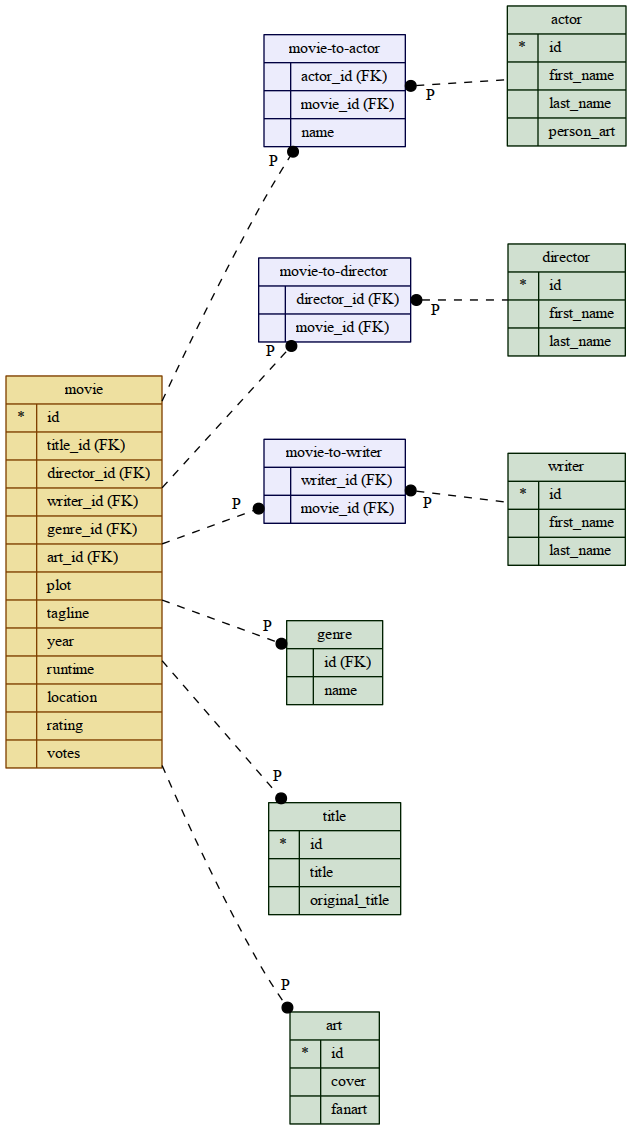
\includegraphics[scale=0.5]{../pics/dataschema}

\subsection{Main View}
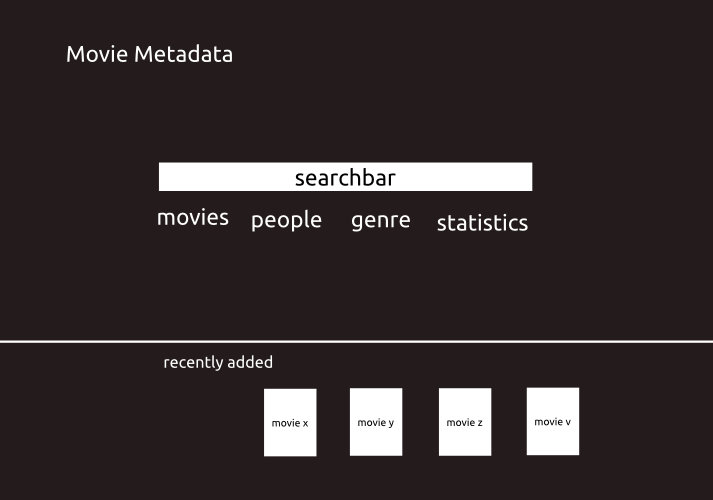
\includegraphics[width=\textwidth]{../pics/mainview}
\paragraph{Inhalt:}
\begin{itemize}
    \item Hauptseite mit Suchfunktion
    \item Kürzlich hinzugefügte Filme anzeigen
    \item Links zur \emph{Movies}, \emph{Genre}, \emph{Persons} und \emph{Statistics} Seite
\end{itemize}

\subsection{Movie View}
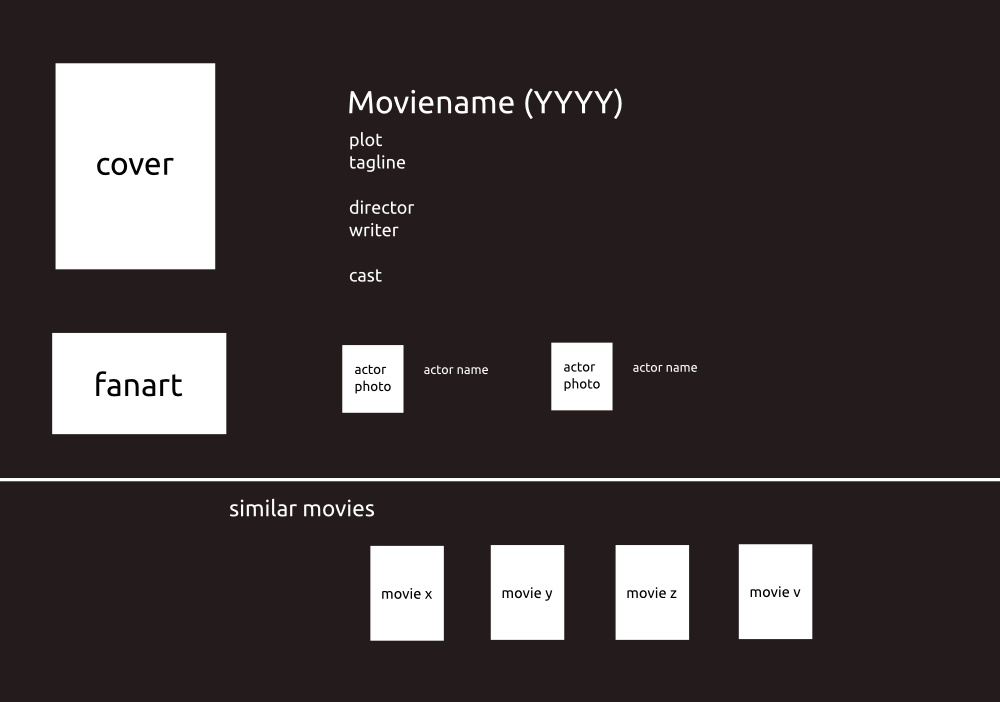
\includegraphics[width=\textwidth]{../pics/movieview}
\paragraph{Inhalt:}
\begin{itemize}
    \item Anzeige von Film-Metadaten, Poster-Art, Fan-Art, Crew und Cast Informationen im oberen Bereich
    \item Anzeige von ,,Similar Movies'' im unteren Bereich
    \item Cast/Crew und Similar Movies leiten auf die jeweilige spezialisierte Seite weiter
\end{itemize}

\subsection{Person View}
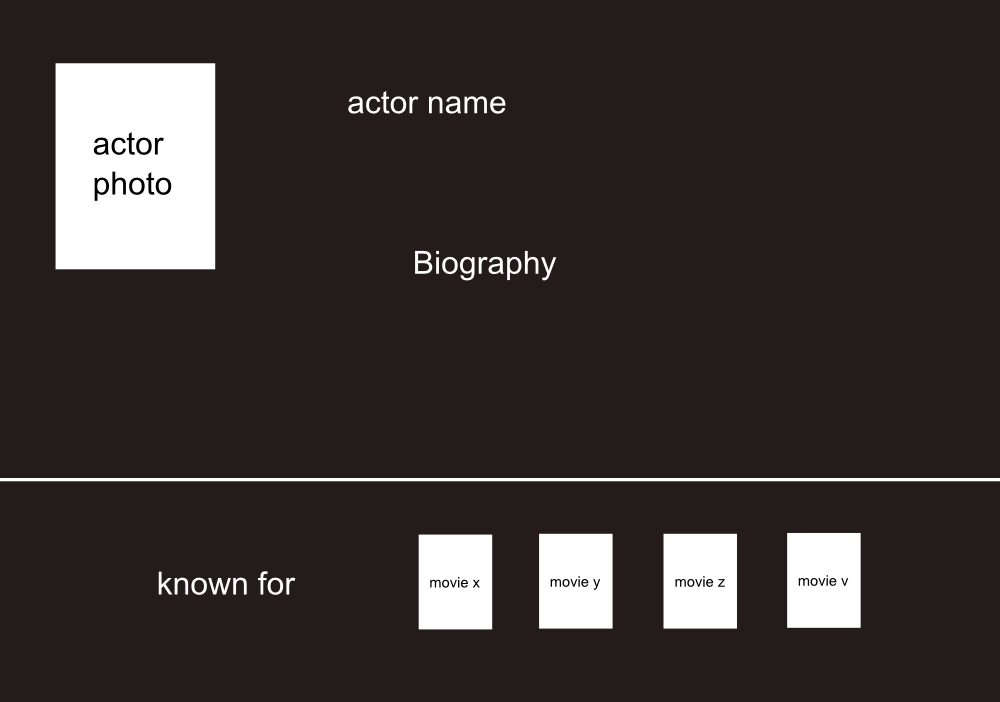
\includegraphics[width=\textwidth]{../pics/actorview}
\paragraph{Inhalt:}
\begin{itemize}
    \item Anzeigen von Schauspieler-Photo und Biografie im oberen Bereich
    \item Anzeigen von Filmen in denen der Schauspieler mitspielt im unteren Bereich
\end{itemize}

\subsection{Statistics}
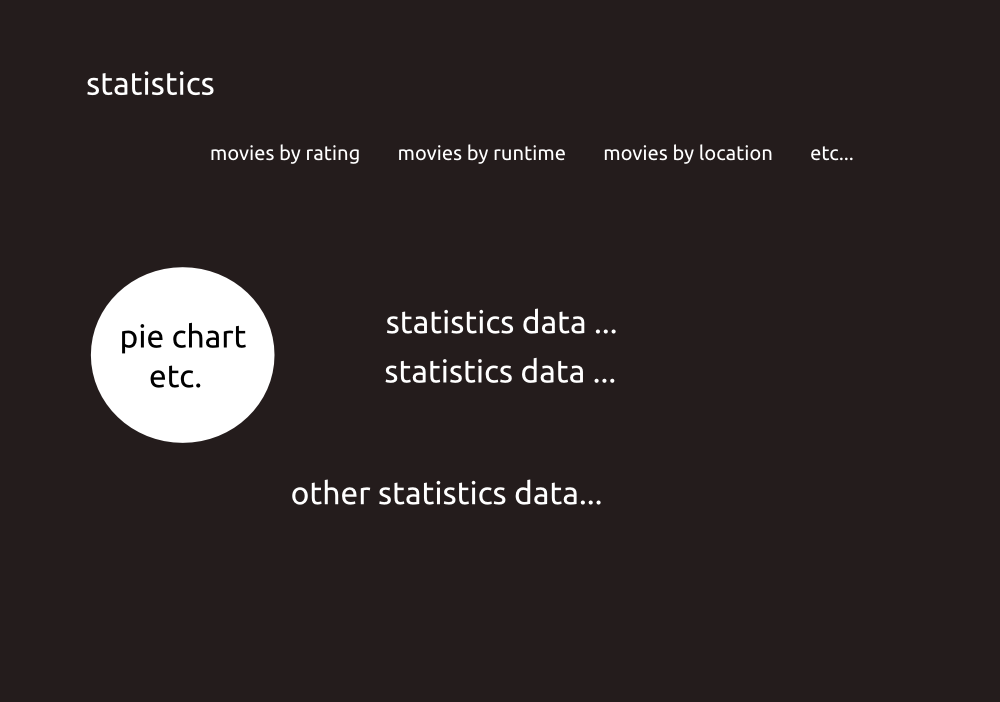
\includegraphics[width=\textwidth]{../pics/statistics}
\paragraph{Inhalt:}
Anzeige von verschiedenen Statistiken wie z.B.:
\begin{itemize}
    \item Liste der besten/schlechtesten Filme
    \item Statistische Auswertung nach Laufzeit, Herstellungsland, Rating, etc.
    \item Genre Charts (z.B. Tortendiagramm)
    \item Person Charts nach Filmgenre
    \item Rating Chart
    \item Statistiken zu gesehenen und eingetragenen Filmen
    \item Favoriten Listen und Statistiken erstellen  
\end{itemize}
